\documentclass[12pt, twoside]{article}
\usepackage[letterpaper, margin=1in, headsep=0.5in]{geometry}
\usepackage[english]{babel}
\usepackage[utf8]{inputenc}
\usepackage{amsmath}
\usepackage{amsfonts}
\usepackage{amssymb}
\usepackage{tikz}
%\usetikzlibrary{quotes, angles}

\usepackage{graphicx}
\usepackage{enumitem}
\usepackage{multicol}

\usepackage{fancyhdr}
\pagestyle{fancy}
\fancyhf{}
\renewcommand{\headrulewidth}{0pt} % disable the underline of the header

\fancyhead[RE]{\thepage}
\fancyhead[RO]{\thepage \\ Name: \hspace{3cm}}
\fancyhead[L]{BECA / Dr. Huson / 10.3 Geometry\\* 3 January 2019}

\begin{document}

\subsubsection*{Classwork: Graphing inequalities \\Due at the end of the period.}
Fill in the values in the blanks and circling the correct types.
  \begin{enumerate}

    \item $\displaystyle y > \frac{4}{3} x -3 $

      \vspace{0.25cm}
      \begin{multicols}{2}
        $y$-intercept $b= \rule{2cm}{0.15mm}$ \\[0.5cm]
        Slope \hspace{0.7cm} $m= \rule{2cm}{0.15mm}$\\[0.5cm]

        Line: \hspace{1cm} Solid ($=$) \hspace{0.5cm} Dashed ($\neq$)\\[0.5cm]
        Shading: \hspace{0.3cm} Above ($y>$) \hspace{0.25cm} Below ($y<$)\\
      \end{multicols}
      Graph the inequality (use a pencil and straight edge - 1 point)

      \begin{center} %4 quadrant regents grid w T-Chart
      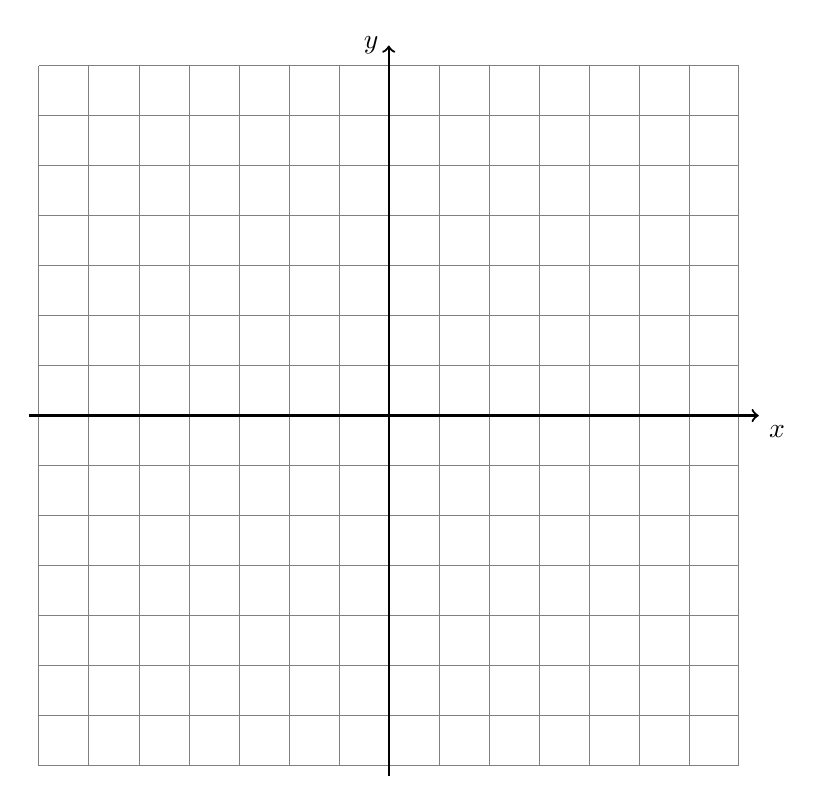
\begin{tikzpicture}[scale=.635]
        \draw [help lines] (-7,-7) grid (7,7);
        \draw [thick, ->] (-7.2,0) -- (7.4,0) node [below right] {$x$};
        \draw [thick, ->] (0,-7.2)--(0,7.4) node [left] {$y$};
      \end{tikzpicture}
      \end{center}

    \item Solve for $y$, then complete. $\displaystyle 4x+ 2y \leq -2 $

        \vspace{2cm}
        \begin{multicols}{2}
          \raggedcolumns
          $y$-intercept $b= \rule{2cm}{0.15mm}$ \\[0.5cm]
          Slope \hspace{0.7cm} $m= \rule{2cm}{0.15mm}$\\

          Line: \hspace{1cm} Solid ($=$) \hspace{0.5cm} Dashed ($\neq$)\\[0.5cm]
          Shading: \hspace{0.3cm} Above ($y>$) \hspace{0.25cm} Below ($y<$)
        \end{multicols}

    \newpage
    \item Graph the two lines after filling in the values in the blanks.\\[0.5cm]


    \begin{multicols}{2}
      $y= -x +5$ \\
      $y=\frac{3}{2} x -5 $
    \end{multicols}
    \begin{multicols}{2}
      \raggedcolumns
      \begin{enumerate}
        \item $y$-intercept $b= \rule{2cm}{0.15mm}$ \\[0.5cm]
        \item Slope \hspace{0.7cm} $m= \rule{2cm}{0.15mm}$\\[0.5cm]
      \end{enumerate}
      \begin{enumerate}
        \item $y$-intercept $b= \rule{2cm}{0.15mm}$ \\[0.5cm]
        \item Slope \hspace{0.7cm} $m= \rule{2cm}{0.15mm}$\\[0.5cm]
      \end{enumerate}
    \end{multicols}

    Label both lines and the solution to the system, the intersection, as a coordinate pair. (3 points) Use pencil for graph (1 point)\\

    \begin{center} %4 quadrant regents grid w T-Chart
    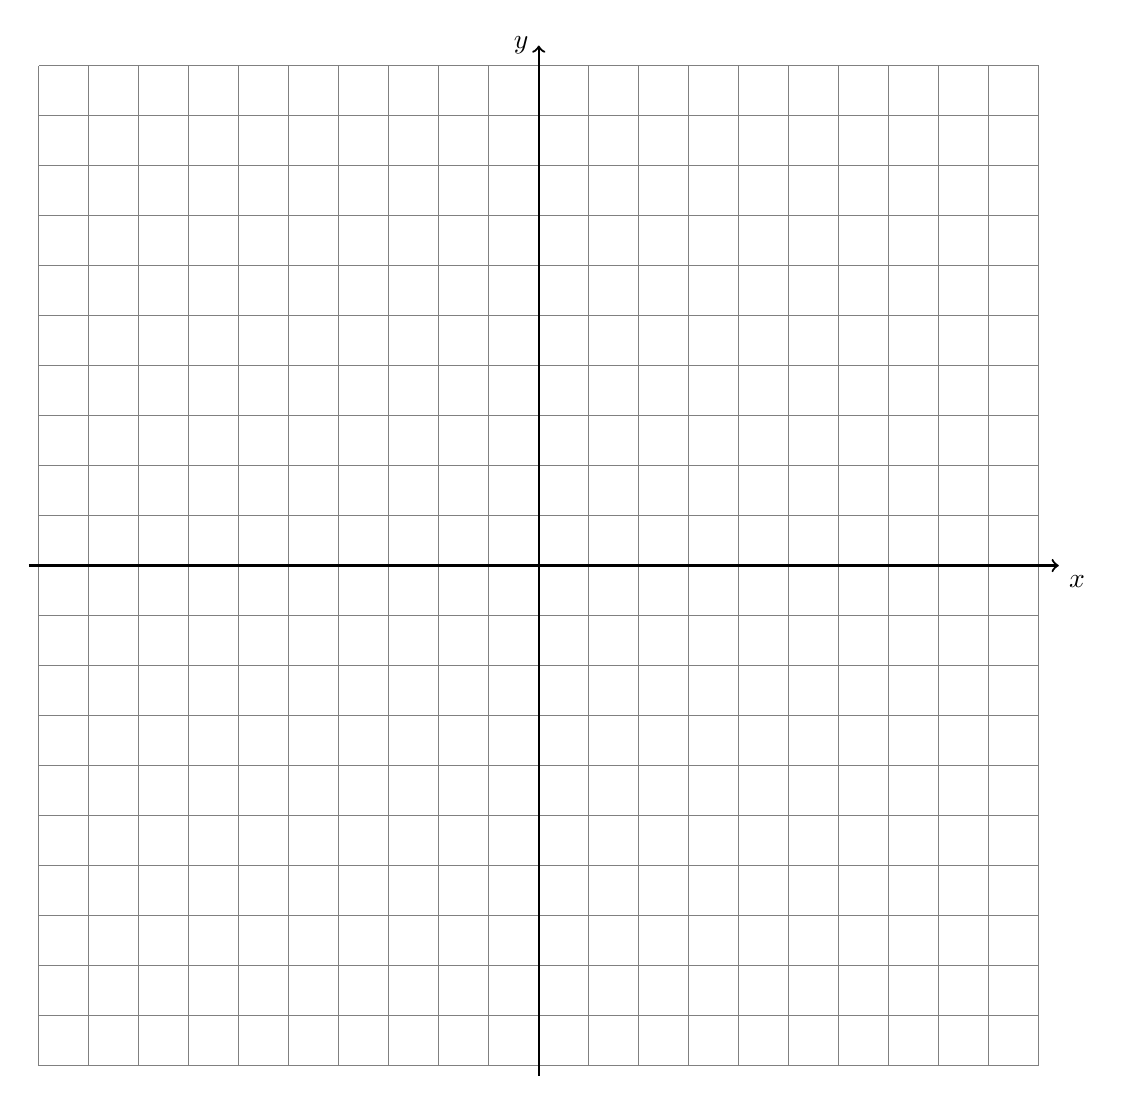
\begin{tikzpicture}[scale=.635]
      \draw [help lines] (-10,-10) grid (10,10);
      \draw [thick, ->] (-10.2,0) -- (10.4,0) node [below right] {$x$};
      \draw [thick, ->] (0,-10.2)--(0,10.4) node [left] {$y$};
    \end{tikzpicture}
    \end{center}

  \newpage
        \subsubsection*{Graphing quadratic functions}

        \item Given the quadratic function $f(x)=x^2-2x$, find the row differences.
          \renewcommand{\arraystretch}{1.6}
            \begin{center}
              \begin{tabular}{|c|r|}
              \hline
              $x$ & $f(x)$\\
              \hline
              -2 & 8 \\
              \hline
              -1 & 3 \\
              \hline
              0 & 0 \\
              \hline
              1 & -1 \\
              \hline
              2 & 0 \\
              \hline
              3 & 3 \\
              \hline
              \end{tabular}
            \end{center}
        Graph the function as a line over the domain $-2 \leq x \leq 3$.

        \begin{center} %4 quadrant regents grid w T-Chart
        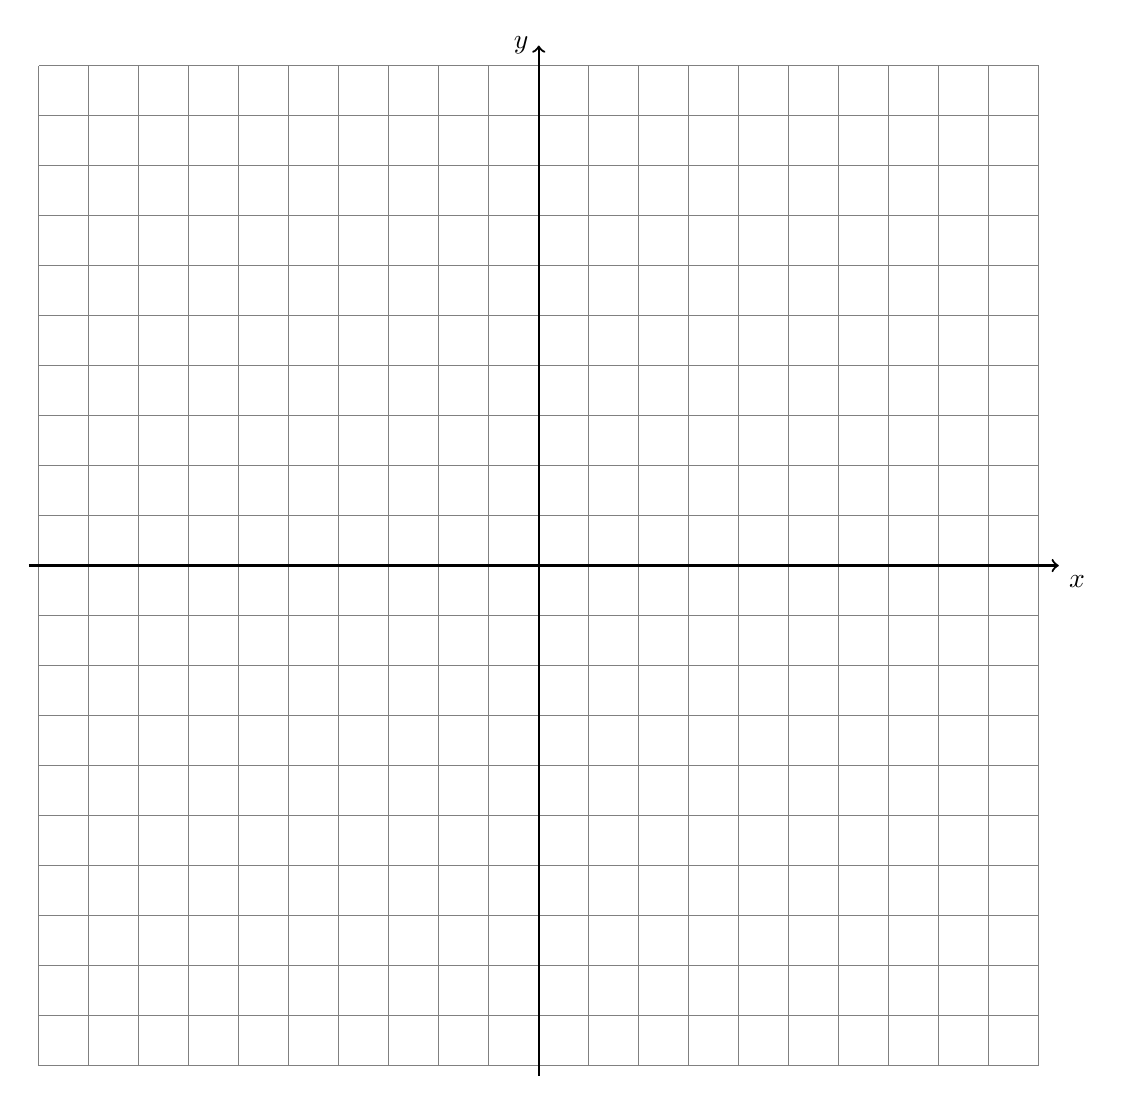
\begin{tikzpicture}[scale=.635]
          \draw [help lines] (-10,-10) grid (10,10);
          \draw [thick, ->] (-10.2,0) -- (10.4,0) node [below right] {$x$};
          \draw [thick, ->] (0,-10.2)--(0,10.4) node [left] {$y$};
        \end{tikzpicture}
        \end{center}
\newpage

    \item Graph the two lines after filling in the values in the blanks.\\[0.5cm]


    \begin{multicols}{2}
      $y= \frac{1}{2} x -5$ \\
      $2x+y = 5 $
    \end{multicols}
    \begin{multicols}{2}
      \raggedcolumns
      \begin{enumerate}
        \item $y$-intercept $b= \rule{2cm}{0.15mm}$ \\[0.5cm]
        \item Slope \hspace{0.7cm} $m= \rule{2cm}{0.15mm}$\\[0.5cm]
      \end{enumerate}
      \begin{enumerate}
        \item $y$-intercept $b= \rule{2cm}{0.15mm}$ \\[0.5cm]
        \item Slope \hspace{0.7cm} $m= \rule{2cm}{0.15mm}$\\[0.5cm]
      \end{enumerate}
    \end{multicols}

    Label both lines and the solution to the system, the intersection, as a coordinate pair. (3 points) Use pencil for graph (1 point)\\

    \begin{center} %4 quadrant regents grid w T-Chart
    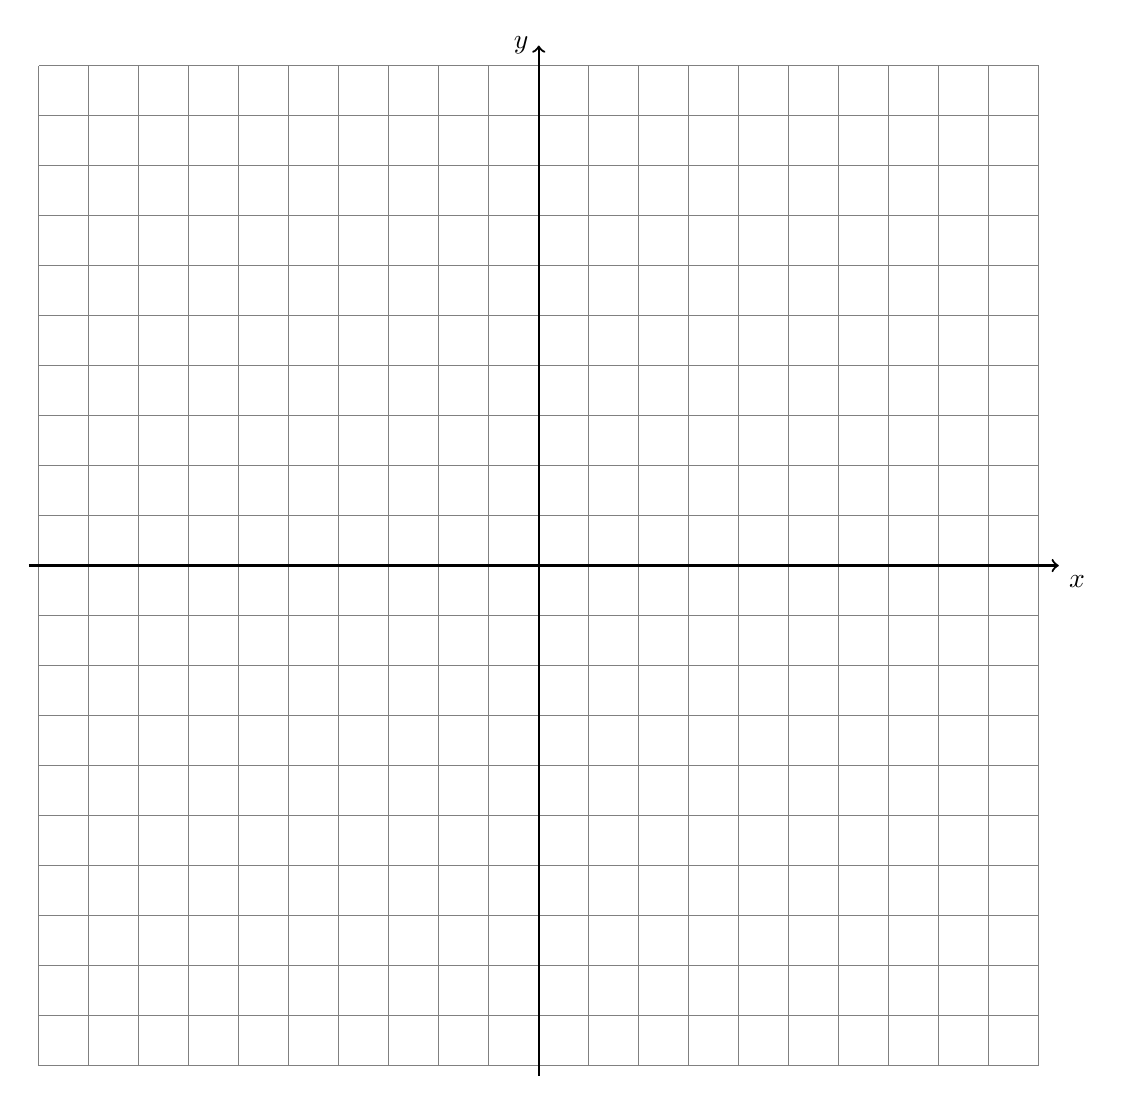
\begin{tikzpicture}[scale=.635]
      \draw [help lines] (-10,-10) grid (10,10);
      \draw [thick, ->] (-10.2,0) -- (10.4,0) node [below right] {$x$};
      \draw [thick, ->] (0,-10.2)--(0,10.4) node [left] {$y$};
    \end{tikzpicture}
    \end{center}

\end{enumerate}

\end{document}

  % problem 35 June 2018
  \item On the set of axes below, graph the following system of inequalities:
    \[2y+3x \leq 14 \]
    \[4x-y < 2\]

    10 by 10 grid

    Determine if the point $(1,2)$ is in the solution set. Explain your answer.

      In the following two problems, solve for the value of $x$.
      \begin{multicols}{2}
      \item   $11=2x+x-1$ \vspace{3cm}
      \item   $\frac{1}{3}(6-3x)=11$ %\vspace{3cm}
      \end{multicols}


    \subsubsection*{Simplify each expression (``Collect like terms")}
      \item $x^2-3x -4 +2x^2+2x+4$ \vspace{1.5cm}
      \item $5(a^2-3a +1) -2(a^2+2a-3)$ \vspace{3cm}
